\documentclass[12pt, notitlepage, final]{article} 

\newcommand{\name}{Vince Coghlan}

%\usepackage[dvips]{graphics,color}
\usepackage{amsfonts}
\usepackage{amssymb}
\usepackage{amsmath}
\usepackage{latexsym}
\usepackage{enumerate}
\usepackage{amsthm}
\usepackage{nccmath}
\usepackage{setspace}
\usepackage[pdftex]{graphicx}
\usepackage{epstopdf}
\usepackage[siunitx]{circuitikz}
\usepackage{tikz}
\usepackage{float}
\usepackage{cancel} 
\usepackage{setspace}
\usepackage{overpic}
\usepackage{mathtools}
\usepackage{listings}
\usepackage{color}
\usepackage{qtree}
%\usepackage{gensymb}

\usetikzlibrary{calc}
\usetikzlibrary{matrix}
\usetikzlibrary{positioning}

\numberwithin{equation}{section}
\DeclareRobustCommand{\beginProtected}[1]{\begin{#1}}
\DeclareRobustCommand{\endProtected}[1]{\end{#1}}
\newcommand{\dbr}[1]{d_{\mbox{#1BR}}}
\newtheorem{lemma}{Lemma}
\newtheorem*{corollary}{Corollary}
\newtheorem{theorem}{Theorem}
\newtheorem{proposition}{Proposition}
\theoremstyle{definition}
\newtheorem{define}{Definition}
\newcommand{\column}[2]{
\left( \begin{array}{ccc}
#1 \\
#2
\end{array} \right)}

\newdimen\digitwidth
\settowidth\digitwidth{0}
\def~{\hspace{\digitwidth}}

\setlength{\parskip}{1pc}
\setlength{\parindent}{0pt}
\setlength{\topmargin}{-3pc}
\setlength{\textheight}{9.0in}
\setlength{\oddsidemargin}{0pc}
\setlength{\evensidemargin}{0pc}
\setlength{\textwidth}{6.5in}
\newcommand{\answer}[1]{\newpage\noindent\framebox{\vbox{{\bf ECEN 5018 Spring 2014} 
\hfill {\bf \name} \vspace{-1cm}
\begin{center}{Project Proposal}\end{center} } }\bigskip }

\DeclareMathOperator*{\argmin}{arg\,min}

%absolute value code
\DeclarePairedDelimiter\abs{\lvert}{\rvert}%
\DeclarePairedDelimiter\norm{\lVert}{\rVert}
\makeatletter
\let\oldabs\abs
\def\abs{\@ifstar{\oldabs}{\oldabs*}}
%
\let\oldnorm\norm
\def\norm{\@ifstar{\oldnorm}{\oldnorm*}}
\makeatother

\def\dbar{{\mathchar'26\mkern-12mu d}}
\def \Frac{\displaystyle\frac}
\def \Sum{\displaystyle\sum}
\def \Int{\displaystyle\int}
\def \Prod{\displaystyle\prod}
%\def \P[x]{\Frac{\partial}{\partial x}}
%\def \D[x]{\Frac{d}{dx}}
\newcommand{\PD}[2]{\frac{\partial#1}{\partial#2}}
\newcommand{\PF}[1]{\frac{\partial}{\partial#1}}
\newcommand{\DD}[2]{\frac{d#1}{d#2}}
\newcommand{\DF}[1]{\frac{d}{d#1}}
\newcommand{\fix}[2]{\left(#1\right)_#2}
\newcommand{\ket}[1]{|#1\rangle}
\newcommand{\bra}[1]{\langle#1|}
\newcommand{\braket}[2]{\langle #1 | #2 \rangle}
\newcommand{\bopk}[3]{\langle #1 | #2 | #3 \rangle}
\newcommand{\Choose}[2]{\displaystyle {#1 \choose #2}}
\newcommand{\proj}[1]{\ket{#1}\bra{#1}}
\def\del{\vec{\nabla}}
\newcommand{\avg}[1]{\langle#1\rangle}
\newcommand{\piecewise}[4]{\left\{\beginProtected{array}{rl}#1&:#2\\#3&:#4\endProtected{array}\right.}
\newcommand{\systeme}[2]{\left\{\beginProtected{array}{rl}#1\\#2\endProtected{array}\right.}
\def \KE{K\!E}
\def\Godel{G$\ddot{\mbox{o}}$del}

%\onehalfspacing

\begin{document}

\answer{}
The basic 9x9 sudoku puzzle can be seen to be a potential game.  If each empty square is a player
in a game, with a utility determined by the amount of repetitions in a row, column, and square, we
can see that if a player makes a move to increase the amount of repetitions in a row, then that other
player in that row will also incur the same costs of repetitions.  This idea of effecting everyone
else the exact same as they effect you gives rise to a potential game.  We can find the potential function
as half of the amount of repetitions of everyone on the board.  This is because if you were to raise your
repetitions by 1, you are increaseing someone else's repititions by one.  That is a total of 2 increases in
global utility, and to maintain the equals sign that defines a potential game, we need it to be a 1 to 1 ratio.
For a group of players $N$ and an action $a\in\mathcal{A}$, we can find that the potential function is:
\[
  \Phi = \frac{1}{2}\sum_{i\in N}U_i(a)
\]

This means that, for a temperature $T>0$, implementing log-linear learning will induce a markov chain with a
unique stationary distrobution of the form:
\[
  \pi_a = \frac{e^{\frac{1}{T}\Phi(a)}}{\sum_{\tilde{a}\in\mathcal{A}}e^{\frac{1}{2}\Phi(\tilde{a})}}
\]
Knowing that a unique stationary distrobution can be found leads to some important questions.  What about games
with multiple solutions?  How quickly will we arrive at this solution?  What temperature will bring us there the
fastest?  What will happen in puzzles without solutions?  Is this solution the stochastically stable state?  Can
we implement a more efficient solver by time-varying the temperature?  Are there other learning algorithms that
will give similar results?

I have implemented this log-linear learning solver in MATLAB, and it can solve most easy puzzles in a fairly short
amount of time.  For example, the following puzzle and soltion is usually solved within 50-100 iterations using
a temperature of $\frac{1}{2}$:

\begin{figure}[H]
\begin{center}
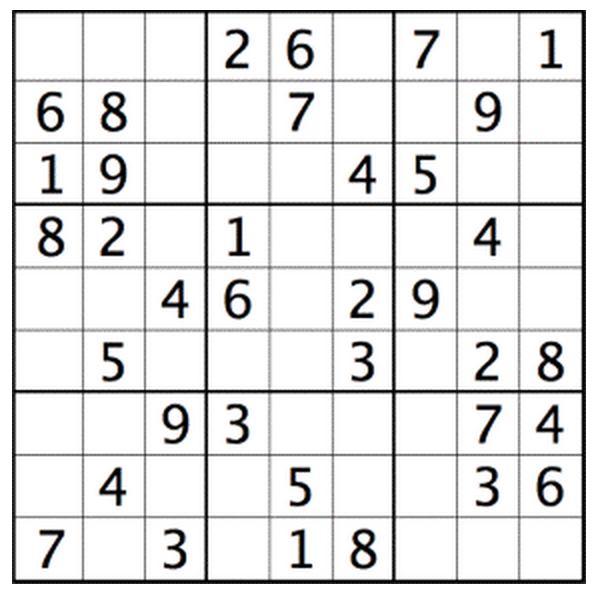
\includegraphics[width=5cm]{f1}
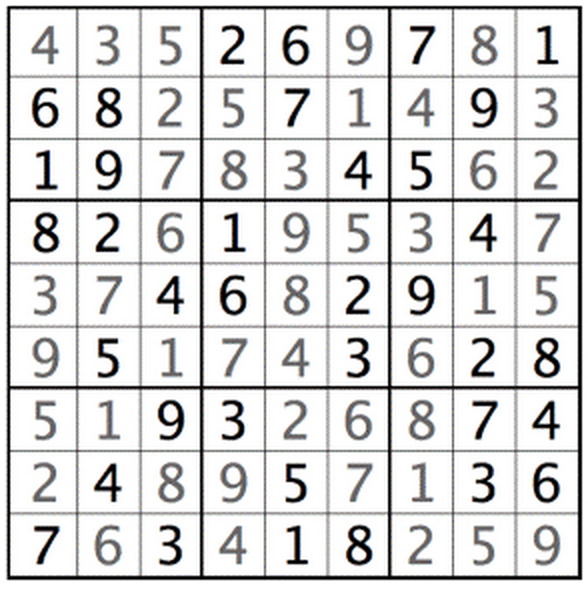
\includegraphics[width=5cm]{f2}
\end{center}
\end{figure}

This is a graph of the iteration versus the amount of rows, columns, and squares that are complete.

\begin{figure}[H]
\begin{center}
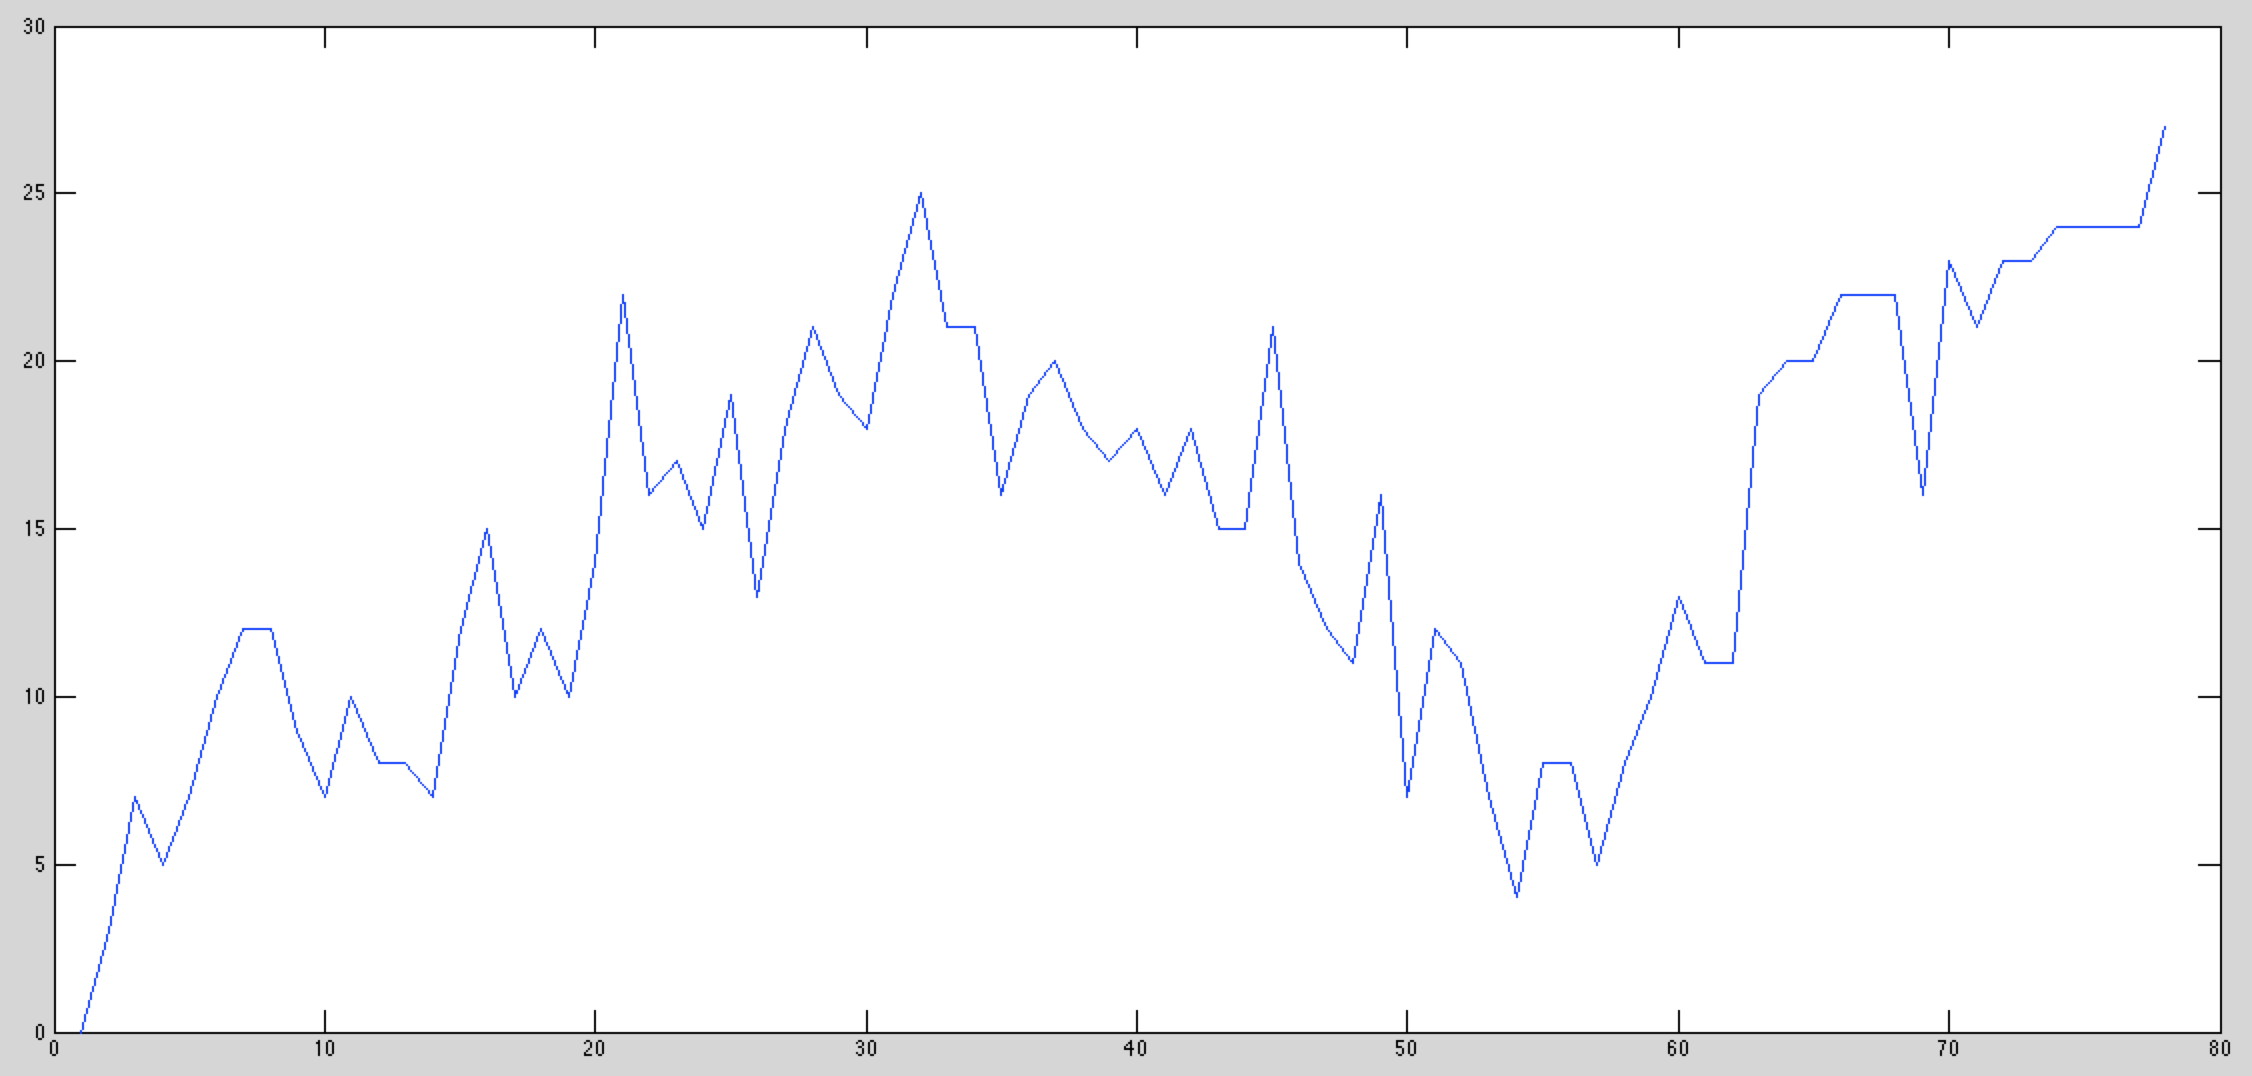
\includegraphics[width=10cm]{f3}
\end{center}
\end{figure}
At 27, we are solved, since 27 is every row, column, and square complete.  The potential can be seen below:
\begin{figure}[H]
\begin{center}
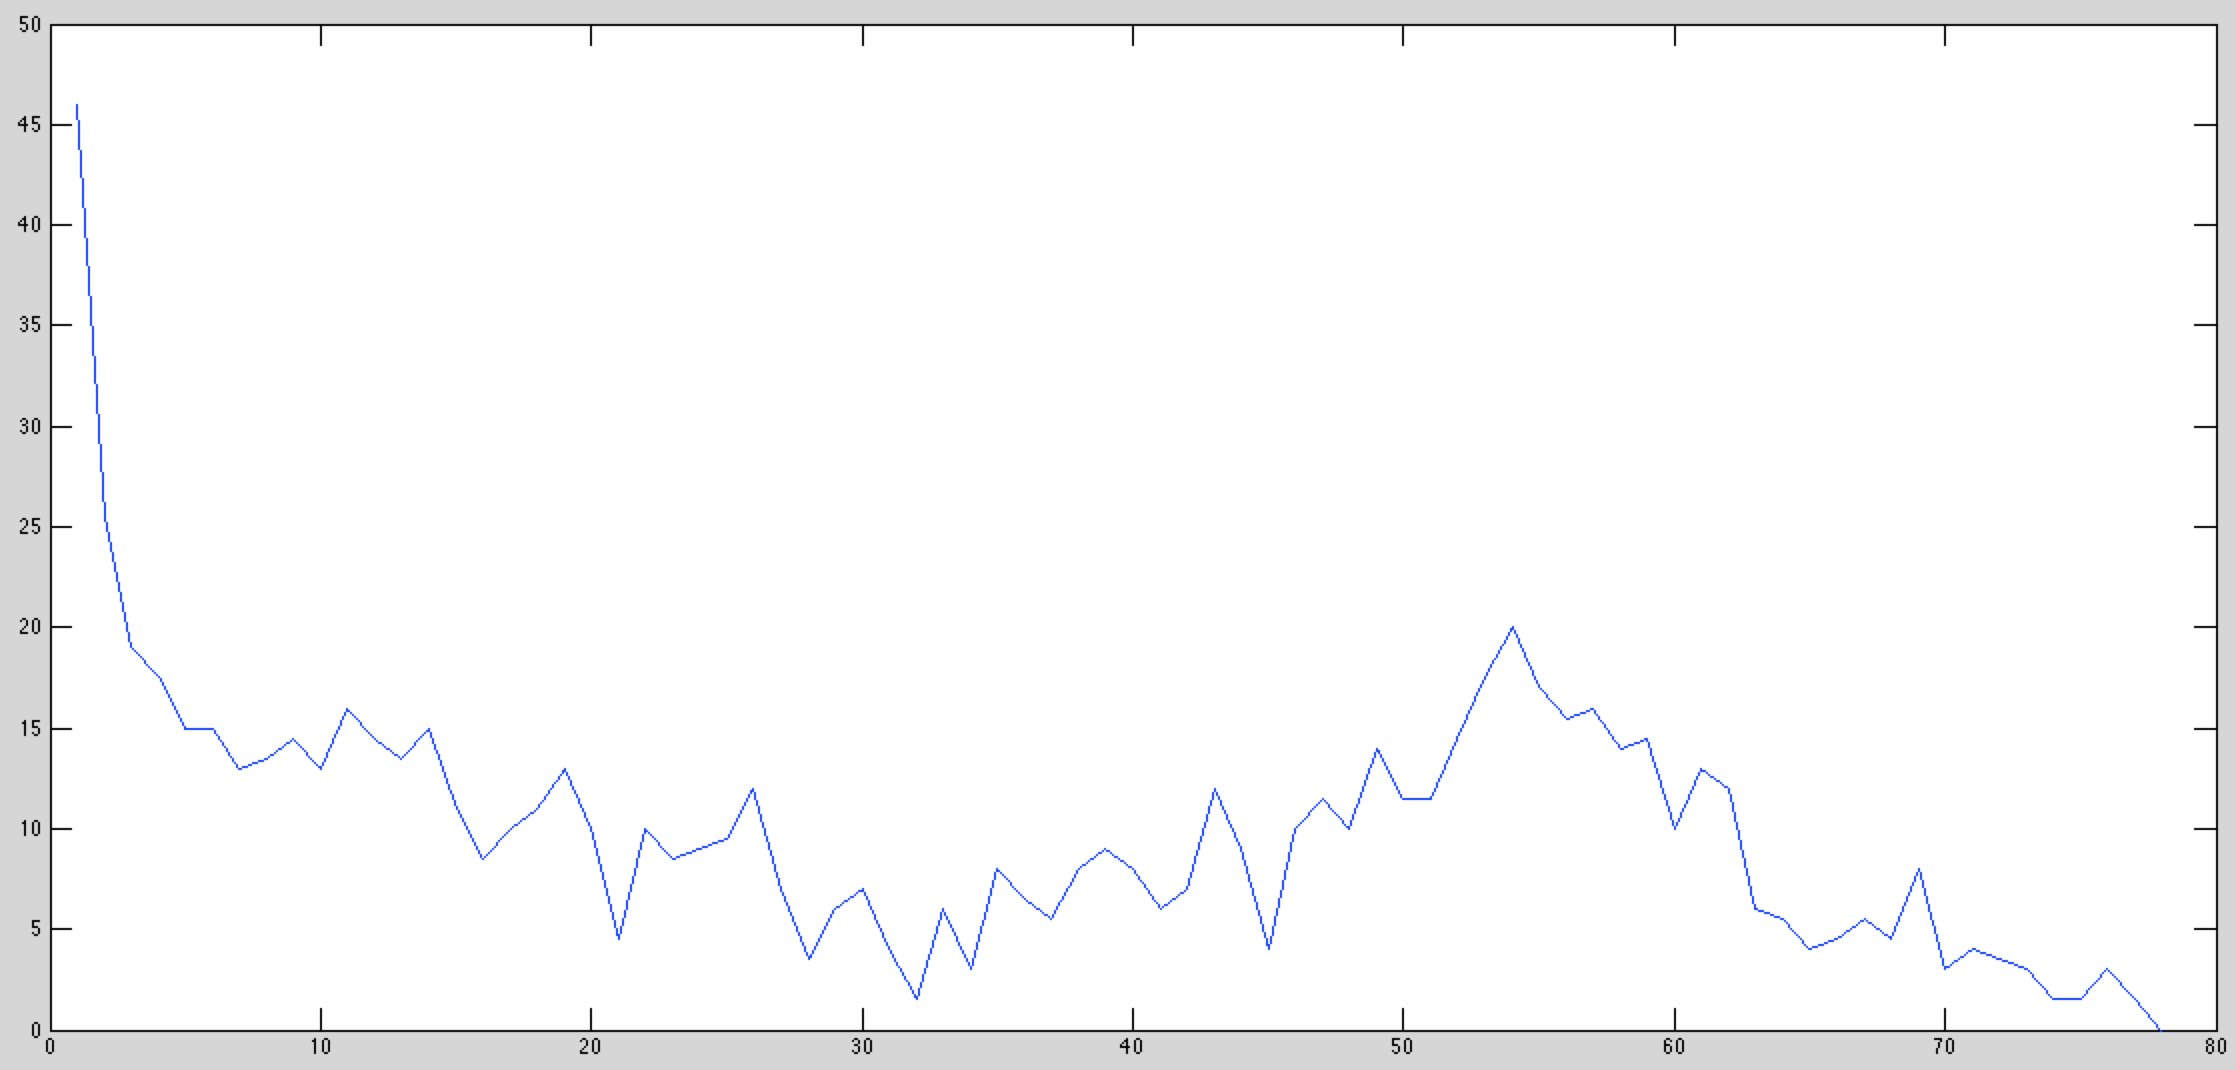
\includegraphics[width=10cm]{f4}
\end{center}
\end{figure}

Here is another example that took 233 iterations to solve:

\begin{figure}[H]
\begin{center}
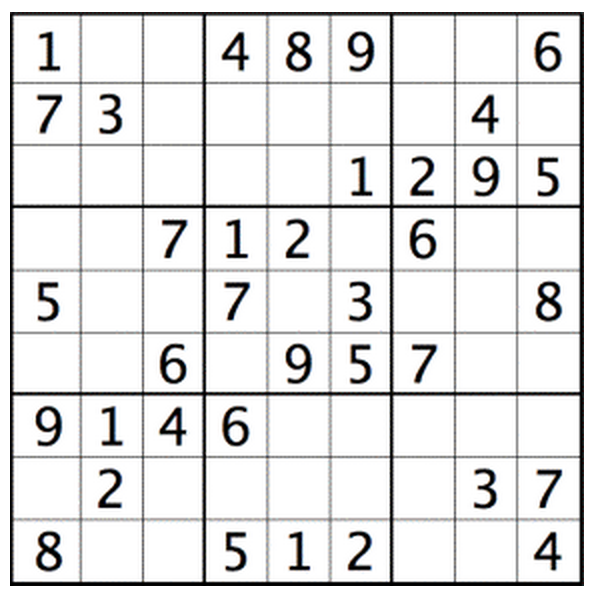
\includegraphics[width=5cm]{f5}
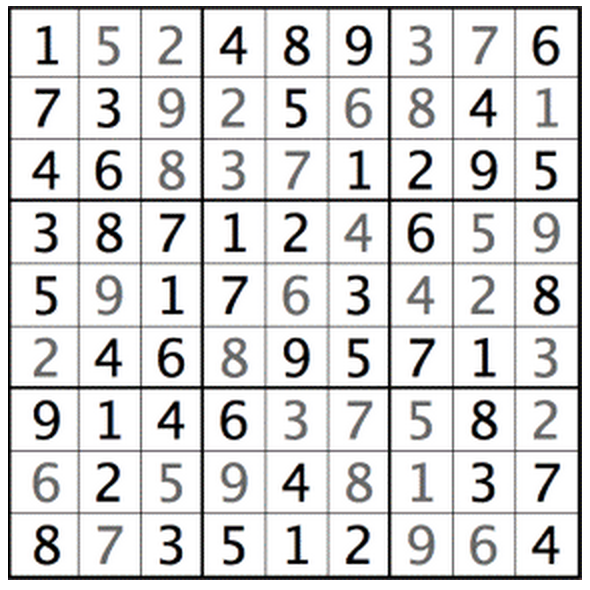
\includegraphics[width=5cm]{f6}
\end{center}
\end{figure}
\begin{figure}[H]
\begin{center}
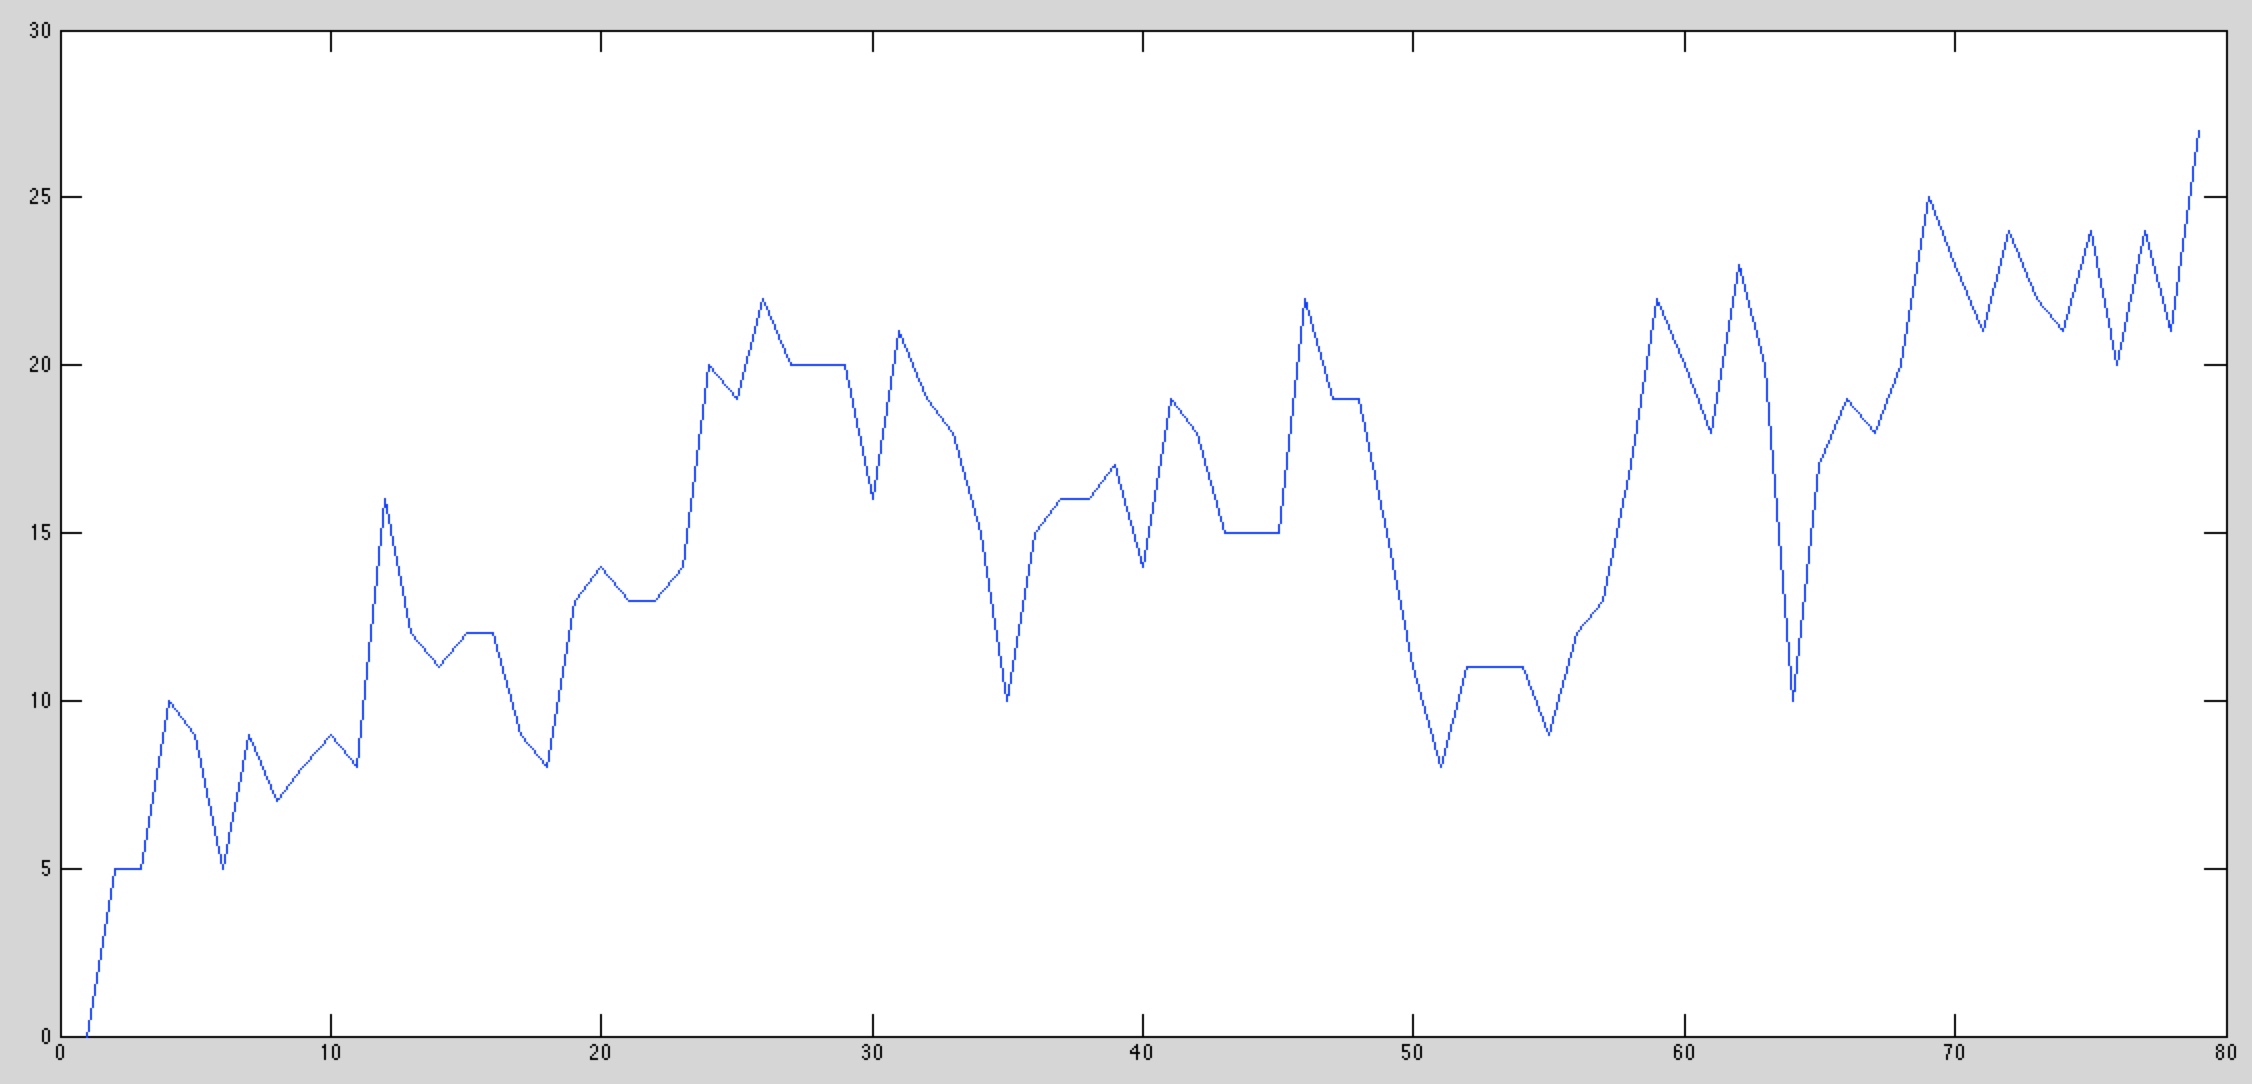
\includegraphics[width=10cm]{f7}
\end{center}
\end{figure}
\begin{figure}[H]
\begin{center}
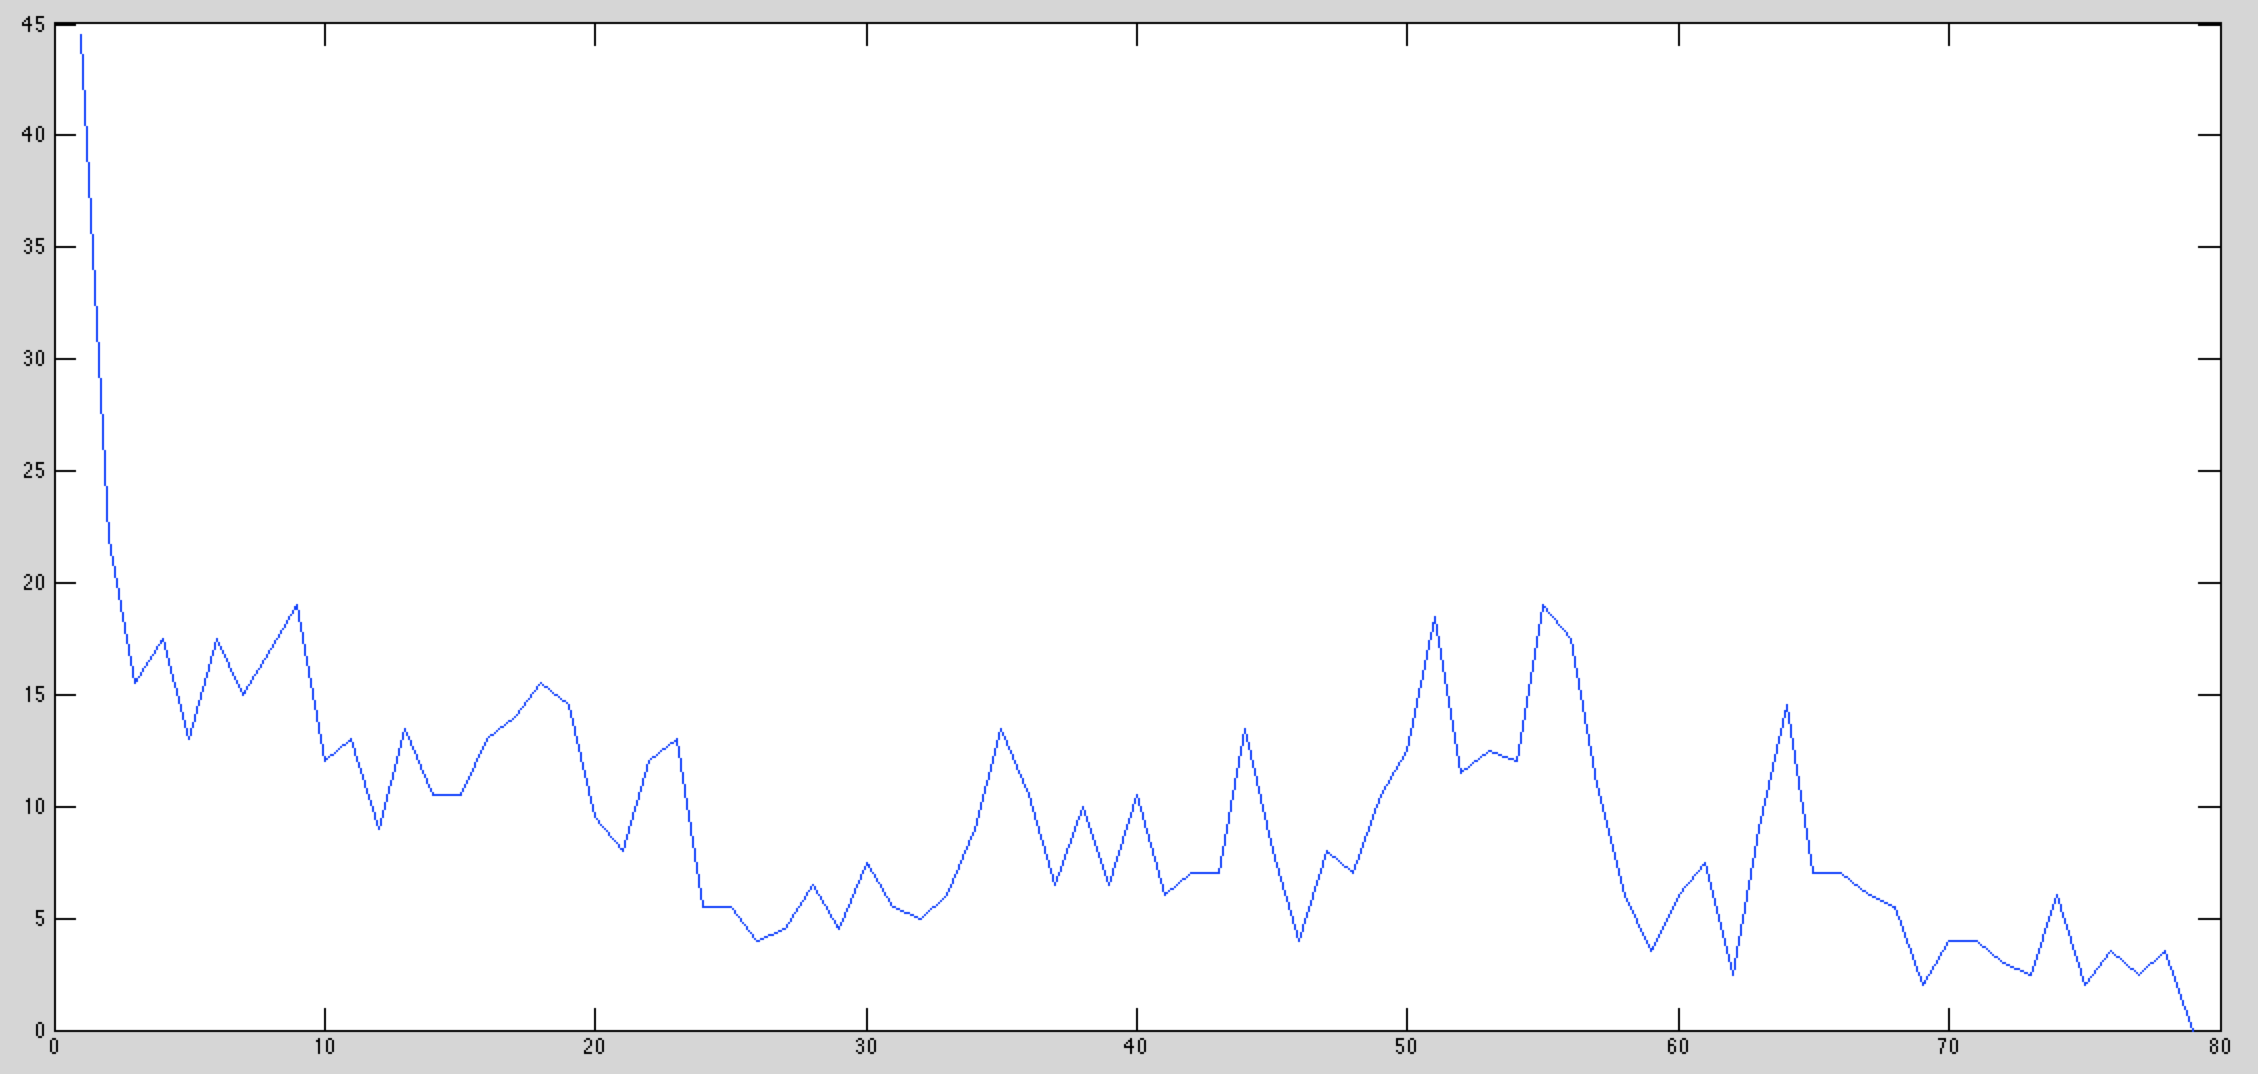
\includegraphics[width=10cm]{f8}
\end{center}
\end{figure}


You can see as it gets very close to the solution, then decides that isnt it and gains chaos again, before settling down to
a new state.  Eventually, it must reach the point of highest potential, which is where we find the solution.  This seems to
work for easy puzzles and select others, but once we pick a difficult puzzle, the amount of iterations it would take seem to
exceed a reasonable amount of computation.  For example, the following puzzle:
\begin{figure}[H]
\begin{center}
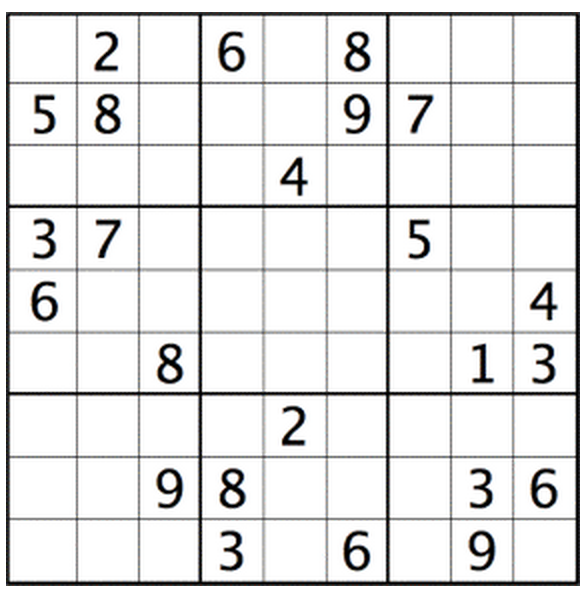
\includegraphics[width=5cm]{f9}
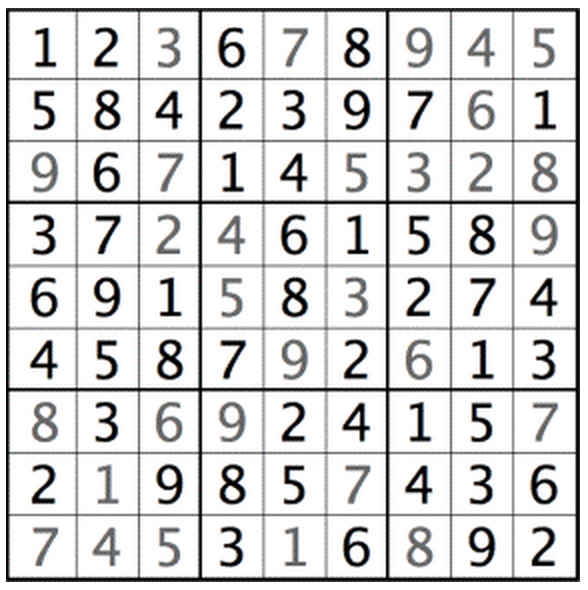
\includegraphics[width=5cm]{f10}
\end{center}
\end{figure}
Will not solve in 50000 iterations.  The potential can be seen below

\begin{figure}[H]
\begin{center}
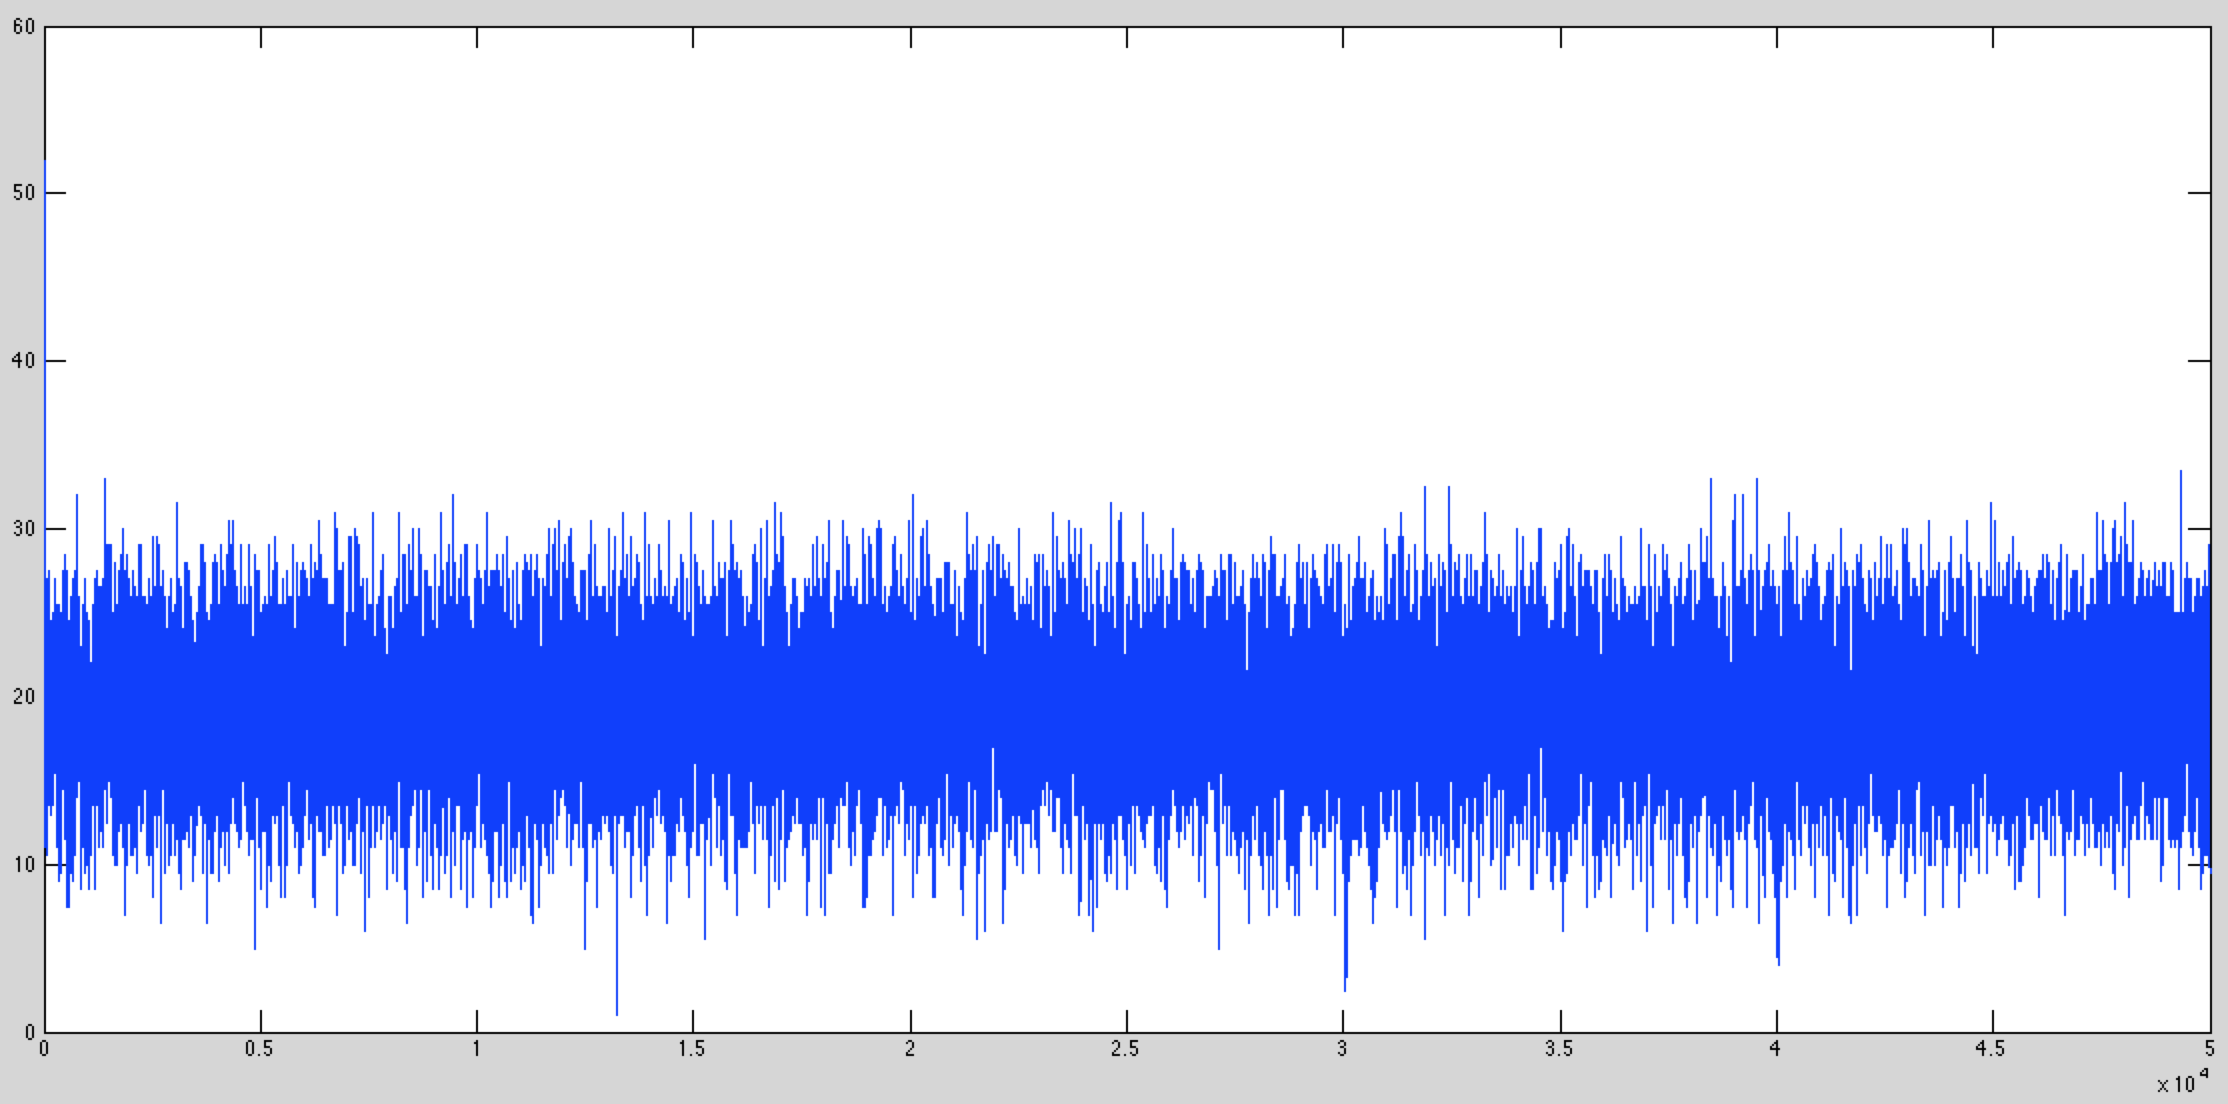
\includegraphics[width=10cm]{f11}
\end{center}
\end{figure}

It gets close sometimes, a value of 2 or 3.  But we never reach the equilibrium.  I think that I may be able to alter LLL to
come up with a method that will solve any sudku puzzle.  Perhaps changing $T$ with time, or maybe a different method of
chosing the player that will chose his move.  In any case, I think this problem can be solved.

What is intreging is that it either takes less than 200-300 iterations, or it takes more than 50000.  There must be a reason
behind this.

\end{document}
